
\section{Introducing Strings}
The grammar evolved
to have more constants 
\begin{center}
\begin{Gcode}[]
<String_abc> ::=  
               | a <String_abc> 
               | b <String_abc>
               | c <String_abc> 
\end{Gcode}
\end{center}
So this grammar accepts \emph{aabaabcac} 
but would reject \emph{adabb} since `d' is not in the list of productions 
rules.  The first line which is blank means this grammar also accepts the 
empty string, often denoted 
$\epsilon$.  We can draw the accepted words as a graph with each vertex 
being an already accepted word and an arrow indicated which production rule 
advanced it to another accepted rule.  The word graph is an infinite 
3-regular tree, of which we show just a snippet.
\begin{center}
    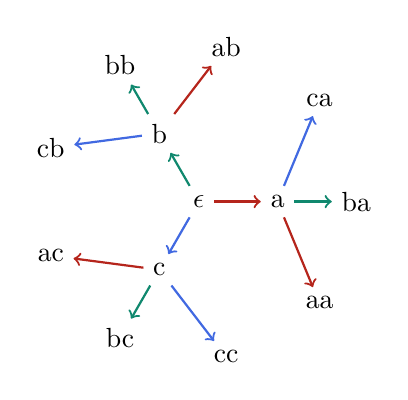
\begin{tikzpicture}
        \node (e) at (0,0) {$\epsilon$};
        \node (a) at (0:1) {a};
        \node (b) at (120:1) {b};
        \node (c) at (240:1) {c};
        \node (aa) at (-40:2) {aa};
        \node (ba) at (0:2) {ba};
        \node (ca) at (40:2) {ca};
        \node (ab) at (80:2) {ab};
        \node (bb) at (120:2) {bb};
        \node (cb) at (160:2) {cb};
        \node (ac) at (200:2) {ac};
        \node (bc) at (240:2) {bc};
        \node (cc) at (280:2) {cc};
    
        \draw[thick,->,BrickRed] (e) -- (a);
        \draw[thick,->,PineGreen] (e) -- (b);
        \draw[thick,->,RoyalBlue] (e) -- (c);
    
        \draw[thick,->,BrickRed] (a) -- (aa);
        \draw[thick,->,PineGreen] (a) -- (ba);
        \draw[thick,->,RoyalBlue] (a) -- (ca);
    
        \draw[thick,->,BrickRed] (b) -- (ab);
        \draw[thick,->,PineGreen] (b) -- (bb);
        \draw[thick,->,RoyalBlue] (b) -- (cb);
    
        \draw[thick,->,BrickRed] (c) -- (ac);
        \draw[thick,->,PineGreen] (c) -- (bc);
        \draw[thick,->,RoyalBlue] (c) -- (cc);
    \end{tikzpicture}
\end{center}
We are in a sense building up new words from old words, 
a form of induction where we have some bases case (the empty word)
and three inductive operators: prepend \code{a}, prepend \code{b}, or 
prepend \code{c}.
Notice because we only pre-pend there is no ambiguity 
in this grammar, that is, $abc$ can only mean $a(bc)$.
% Similar to the natural numbers, strings are the type 
% of another algebra, a \emph{free monoid} it will be called.
% This will become the start of a future algebra is another algebra, with one nullary operator 
% $\epsilon$ and three unary operators {\color{BrickRed}a$\Box$}, 
% {\color{PineGreen}b$\Box$}, and {\color{RoyalBlue}c$\Box$}
% being the production rules, that is the tree colors of arrows.

We can again make this computational.
\begin{Fcode}[]
data String_abc = nil
            | 'a' s:String_abc
            | 'b' s:String_abc
            | 'c' s:String_abc
\end{Fcode}
\begin{Pcode}[]
class StringABC
  case Nil extends StringABC
  case A(tail:String) extends StringABC
  case B(tail:String) extends StringABC
  case C(tail:String) extends StringABC
sealed
\end{Pcode}
    
\index{\code{<<Accept>>}}\index{grammar!accepted}
This all gets a bit tedious as we can see there is a pattern of
\code{<Character> <String>}.  So we remedy this by first we fix an alphabet
separately as its own inductive grammar and make strings that use a variable alphabet.
We need one further adaptation, since we add in new production rules in 
the services our of our main one we now indicated the productions 
that are ultimately acceptable by \code{<<Accept>>}.
\begin{Gcode}[]
<Char> ::= a | b | c | d | e
<<String>> ::= 
           | <Char> <String>
\end{Gcode}
Translated to popular coding styles this might be:
\begin{Fcode}[]
data AB = a | b
data ABC = a | b | c 
data String Char = Empty 
            | Prepend( head:Char, tail:String) 
a2 = a:String AB
a3 = a:String ABC --- a different 'a'
\end{Fcode}
We read \code{String} and now taking a parameter \code{Char}
which we could be any alphabet, but here it is given the 
choice of [a,b] and [a,b,c].
Writing \lstinline{head:Char} or \lstinline{tail:String} 
indicates that head must come from the alphabet we chose 
and tail must be some already produced string, possibly empty.
Some readers might relate to a different dialect of 
programming such as the following
\begin{Pcode}[]
class AB
  case A extends Char;  case B extends Char;
sealed
class ABC
  case A extends Char;  case B extends Char;
  case C extends Char
sealed
class String[Char]
  case Empty extends String
  case Prepend( head:Char, tail:String) extends String
sealed
a2 = new Prepend[AB](a, Empty())
a3 = new Prepend[ABC](a, Empty())
\end{Pcode}
% \end{lstlisting}
Observe the similarities with Peano's natural numbers:
\begin{align}
     2 & \defeq S(S(0)) \tag{$\mathbb{N}$}\\
 \text{\lstinline{"me"}} & \defeq \text{\lstinline{Prepend('m',Prepend('e',Empty))}}
\tag{String}
\end{align}
The left-hand sides are merely notation for what the data really is on the right.
Both the successor and the \lstinline{Prepend} are operators that generate 
new values.  Later in you shall come to know these constructions as free algebras,
but they are also foundational to programming.



\begin{remark}{Dictionaries and Sentences}
    The above examples demonstrate how the language of grammars came to 
    use terms like ``alphabet/word''. 
    In natural languages however, the building blocks of grammar are comprised of words (or
    at least syllables), as would be found in a dictionary, not an alphabet.  
    Likewise the grammar clarifies what it means to accept a string of words as a sentence,
    not what words are in the language. This offset in vocabulary better 
    approximates the tradition of languages like Chinese
    where entire words can be characters in the alphabet and strings of
    characters are sentences.
\end{remark}
